\documentclass{beamer}

\usetheme{AAUsimple}

\usepackage{amsmath,amssymb,graphicx}
\usepackage{tikz}
\usetikzlibrary{matrix,arrows,decorations,decorations.markings,tikzmark,fit,shapes.geometric,decorations.pathmorphing,backgrounds}
\usepackage{listings}
\usepackage{upquote}
\newcounter{ipythoncounter}
\setcounter{ipythoncounter}{1}
\renewcommand{\ttdefault}{pcr}
\lstset{
  aboveskip=\bigskipamount,
  belowskip=\bigskipamount,
  basicstyle=\footnotesize\ttfamily,
  language=Python,
  numbers=left,
  stepnumber=9999,
  numberfirstline=true,
  xleftmargin=2cm,
}

\lstnewenvironment{ipythoninput} {
  \setcounter{lstnumber}{\value{ipythoncounter}} \renewcommand{\thelstnumber}
             {\bf\ttfamily In [\the\value{ipythoncounter}]:} \lstset{
               frame=single, frameround=tttt, name=ipythoninput, } } {
  \addtocounter{ipythoncounter}{1} }

\lstnewenvironment{ipythonoutput} { \addtocounter{ipythoncounter}{-1}
  \setcounter{lstnumber}{\value{ipythoncounter}} \renewcommand{\thelstnumber}
             {\bf\ttfamily Out[\the\value{ipythoncounter}]:} \lstset{
               name=ipythoninput } } { \addtocounter{ipythoncounter}{1} }


\DeclareMathOperator{\ZZ}{\mathbb{Z}}
\DeclareMathOperator{\RR}{\mathbb{R}}
\DeclareMathOperator{\CC}{\mathbb{C}}
\DeclareMathOperator{\hg}{\mathfrak{h}_g}
\newcommand{\dx}{\,\mathrm{d}x}
\newcommand{\dt}{\,\mathrm{d}t}
\newcommand{\dQ}{\,\mathrm{d}Q}
\DeclareMathOperator{\DivC}{\mathcal{C}}
\DeclareMathOperator{\DivD}{\mathcal{D}}
\DeclareMathOperator{\RCV}{\boldsymbol{K}}
\DeclareMathOperator{\Abel}{\boldsymbol{A}}
\DeclareMathOperator{\HalfLattice}{\Lambda_{1/2}}

\newcommand{\thchar}[2] {\begin{bmatrix}#1\\#2\end{bmatrix}}
\newcommand{\thcharsm}[2] {\left[ \begin{smallmatrix} #1
      \\ #2 \end{smallmatrix} \right]}



%%%%%%%%%%%%%%%%%%%%%%%%%%%%%%%%%%%%%%%%%%%%%%%%%%%%%%%%%%%%%%%%%%%%%%%%%%%%%%%
\title{Computing Solutions to the Kadomtsev--Petviashvili Equation}

\author{
  Chris Swierczewski\\
  {\tt cswiercz@uw.edu}
}

\date{9 January 2016}

\institute{
  Department of Applied Mathematics\\
  University of Washington\\
  Seattle, Washington
}

\pgfdeclareimage[height=1.5cm]{titlepagelogo}{AAUgraphics/aau_logo_new_circle}
\titlegraphic{
  \pgfuseimage{titlepagelogo}
}

%%%%%%%%%%%%%%%%%%%%%%%%%%%%%%%%%%%%%%%%%%%%%%%%%%%%%%%%%%%%%%%%%%%%%%%%%%%%%%%



%%%%%%%%%%%%%%%%%%%%%%%%%%%%%%%%%%%%%%%%%%%%%%%%%%%%%%%%%%%%%%%%%%%%%%%%%%%%%%%%
\begin{document}
%%%%%%%%%%%%%%%%%%%%%%%%%%%%%%%%%%%%%%%%%%%%%%%%%%%%%%%%%%%%%%%%%%%%%%%%%%%%%%%%


\begin{frame}[plain,noframenumbering]
  \titlepage
\end{frame}

\begin{frame}{Acknowledgements}{}
  \begin{itemize}
  \item Bernard Deconinck
  \item Daniel Shapero
  \item National Science Foundation Grant NSF-DMS-1008001
  \end{itemize}
\end{frame}

\begin{frame}{Kadomtsev--Petviashvili Equation}{}
  $u(x,y,t) = $ surface height of a 2D shallow water wave,
  \[
  \tfrac{3}{4} u_{yy} = \frac{\partial}{\partial x} \left(
  u_t - \tfrac{1}{4} \left(6uu_x + u_{xxx}\right) \right).
  \]
  {\it \small Only considering periodic solutions.}
  \begin{columns}[T]
    \begin{column}{0.5\textwidth}
      \begin{figure}
        \centering
        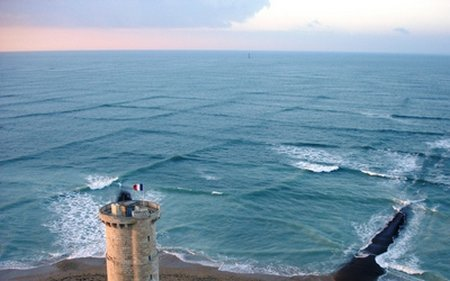
\includegraphics[width=\textwidth]{images/livekp.jpg}
        \caption{\^{I}le de R\'{e}, France}
      \end{figure}
    \end{column}
    \begin{column}{0.5\textwidth}
      \begin{figure}
        \centering
        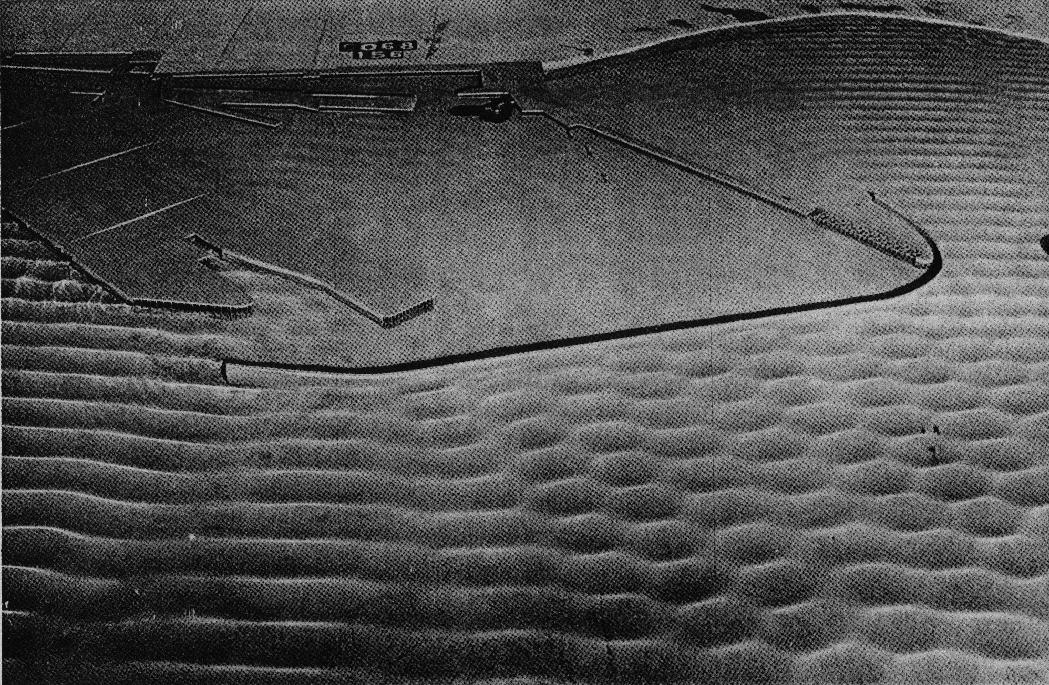
\includegraphics[width=0.96\textwidth]{images/sd-harbor-model.jpg}
        \caption{Model of San Diego Harbor}
      \end{figure}
    \end{column}
  \end{columns}
\end{frame}


\begin{frame}{Finite Genus Solutions}{}
  \[
  u(x,y,t)
  =
  2c + 2 \partial_x^2
  \log \theta
  \Big(
  \boldsymbol{U}x + \boldsymbol{V}y + \boldsymbol{W}t + \boldsymbol{D},
  \Omega
  \Big)
  \]

  \vspace{24pt}
  \pause
  
  \begin{overprint}

    %%%%%%%%%%%%%%%%%%%%
    \onslide<+>
    
    Riemann theta function,
    \[
    \theta : \CC^g \times \hg \to \CC
    \]
    where $\hg =$ space of {\it Riemann matrices}:
    \begin{itemize}
    \item $\Omega \in \CC^{g \times g}$,
    \item $\Omega^T = \Omega$,
    \item $\text{Imag}(\Omega) > 0$.
    \item ($g =$ ``genus'')
    \end{itemize}
    
    %%%%%%%%%%%%%%%%%%%%
    \onslide<+>

    $\boldsymbol{U},\boldsymbol{V},\boldsymbol{W},\boldsymbol{D}\in\CC^g$,
    $\Omega \in \hg$ derived from compact Riemann surface
    \begin{itemize}
    \item {\bf For this talk}: {\it compact Riemann surface} = complex solutions
      to plane algebraic curve
      \vspace{12pt}
      \[
      C = \big\{ (\lambda,\mu) \in \CC^*
             \; \big| \;
             f(\lambda,\mu) = 0, \; f \in \CC[\lambda,\mu] \big\}.
      \]
    \end{itemize}

    %%%%%%%%%%%%%%%%%%%%
    \onslide<+>

    \begin{block}{Goal}
      Given a Riemann surface $X$ and a {\it divisor} $\DivD$ on $X$ compute the
      corresponding solution to the KP equation.
    \end{block}
    \begin{itemize}
    \item {\it Note: solutions not necessarily real or bounded.}
    \end{itemize}
  \end{overprint}
\end{frame}


\begin{frame}[fragile]{Journey to the Initial Value Problem}{}
  \begin{figure}
    \centering
    \begin{tikzpicture}[descr/.style={fill=white}]
      \matrix(m)[matrix of math nodes, row sep=3.5em, column sep=6em,
                 text height=1.5ex, text depth=0.25ex]
             {
               u(x,y,0) & X,\DivD \\
               u(x,y,t) & \boldsymbol{U},\boldsymbol{V},\boldsymbol{W},\boldsymbol{D}, \Omega \\
             };

             \path[->,font=\scriptsize]
             (m-1-1) edge node[auto] {Deconinck} (m-1-2)
             (m-1-1) edge[dashed] node[auto] {} (m-2-1)
             (m-1-2) edge node[near start,right]
                          {A) Krichever, Deconinck, van Hoeij}
                          node[near end, right]
                          {B) Frauendiener, Klein}
                     (m-2-2)
             (m-1-2) edge[dashed] node[descr] {Bobenko} (m-2-1)
             (m-2-2) edge[bend left,dashed] node[auto]
                     {Dubrovin, Flickinger, Segur}
                     (m-2-1)
             (m-2-2) edge node[auto] {Krichever} (m-2-1);

             %%%%%%%%%%%%%%%%%%%%
                          
             \onslide<2>{
               \path[->,font=\scriptsize,ultra thick,color=frametitle.bg]
               (m-2-2) edge node[auto] {Krichever}
                       (m-2-1);
             }
             \onslide<3>{
               \path[->,font=\scriptsize,ultra thick,color=frametitle.bg]
               (m-1-2) edge node[near start,right]
                            {A) Krichever, Deconinck, van Hoeij}
                            node[near end, right]
                            {} %{B) Frauendiener, Klein}
                       (m-2-2);
             }
             \onslide<4>{
               \path[->,font=\scriptsize,ultra thick,color=frametitle.bg]
               (m-1-2) edge node[near start,right]
                            {} %{A) Krichever, Deconinck, van Hoeij}
                            node[near end, right]
                            {B) Frauendiener, Klein}
                       (m-2-2);
             }

             \onslide<5>{
               \path[->,font=\scriptsize,ultra thick,color=frametitle.bg]
               (m-1-1) edge node[auto] {Deconinck}
                       (m-1-2);
             }
             \onslide<6>{
               \path[->,font=\scriptsize,ultra thick,color=frametitle.bg]
               (m-2-2) edge[bend left,dashed] node[auto]
                       {Dubrovin, Flickinger, Segur}
                       (m-2-1);
             }
             \onslide<7>{
               \path[->,font=\scriptsize,ultra thick,color=frametitle.bg]
               (m-1-2) edge[dashed] node[descr] {Bobenko}
                       (m-2-1);
             }
             \onslide<8>{
               \draw [->,ultra thick,color=red]
               (m-1-2.south) .. controls (m-2-2)
                             .. (m-2-1.east);
             }
             \onslide<9>{
               \draw [->,ultra thick,color=red]
               (m-1-1.east) .. controls (m-1-2)
                            .. (2,0)
                            .. controls (m-2-2)
                            .. (m-2-1.east);
             }
    \end{tikzpicture}
  \end{figure}

  \begin{overprint}

    \onslide<2> %%%%%%%%%%%%%%%%%%%%

    \begin{block}{Krichever}
      The finite-genus formulae are indeed solutions to KP. (Where parameters
      are obtained from a Riemann surface.)
    \end{block}

    \onslide<3> %%%%%%%%%%%%%%%%%%%%

    \begin{block}{Krichever, Deconinck, van Hoeij}
      Krichever's inverse procedure + Deconinck / van Hoeij's computational
      framework used to obtain necessary parameters.
    \end{block}

    \onslide<4> %%%%%%%%%%%%%%%%%%%%

    \begin{block}{Frauendiener, Klein}
      {\it Alt. approach: use ``Real Riemann surfaces''.}
    \end{block}

    \onslide<5> %%%%%%%%%%%%%%%%%%%%
    
    \begin{block}{Deconinck}
      Begin with initial condition $u(x,y,0)$ of the form,
      \[
      u(x,y,0)
      =
      2c + 2 \partial_x^2
      \log \theta
      \Big(
      \boldsymbol{u}x + \boldsymbol{v}y + \boldsymbol{d},
      \Omega
      \Big).
      \]
    \end{block}

    \onslide<6> %%%%%%%%%%%%%%%%%%%%
    
    \begin{block}{Dubrovin, Flickinger, Segur}
      {\it Alt. approach: algebraic conditions on parameters.
      \begin{itemize}
      \item Only works in $g=2,3$ case.
      \end{itemize}
      }
    \end{block}

    \onslide<7> %%%%%%%%%%%%%%%%%%%%
    
    \begin{block}{Bobenko}
      {\it Alt. approach: use ``Schottky Uniformization'' techniques.}
    \end{block}

    \onslide<8> %%%%%%%%%%%%%%%%%%%%

    \begin{block}{Goal}
      Realizing the map
      \[
      X,\DivD \quad \longrightarrow \quad u(x,y,t)
      \]
      in Sage using the software package ``Abelfunctions''.
    \end{block}
    
    \onslide<9> %%%%%%%%%%%%%%%%%%%%

    \begin{block}{Future Goal}
      Solving the initial value problem
      \[
      u(x,y,0) \quad \longrightarrow \quad u(x,y,t)
      \]
      in Sage using the software package ``Abelfunctions''.
  \end{block}
    
  \end{overprint}
\end{frame}

\begin{frame}{abelfunctions}{}
  \setbeamercolor{block body}{use={block title},bg=block title.fg}
  \begin{block}{}
  \begin{figure}[t]
    \centering
    
\includegraphics[width=0.9\textwidth]{./images/abelfunctions.png}
  \end{figure}
  \end{block}

  \vspace{16pt}

  A Sage library for computing with Abelian functions, Riemann surfaces, and
  complex algebraic curves.
  \begin{center}
    {\tt https://github.com/cswiercz/abelfunctions}

    {\tt https://www.cswiercz.info/abelfunctions}
  \end{center}
\end{frame}


\begin{frame}{Riemann Surfaces in One Picture}{}
  \begin{figure}
  \centering
  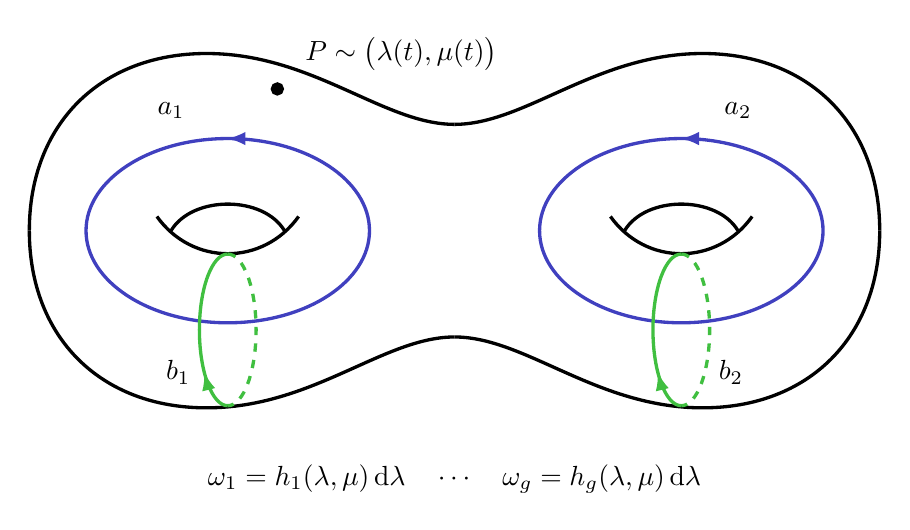
\begin{tikzpicture}[scale=0.9]
    \colorlet{darkgreen}{green!50!gray}
    \colorlet{lightgray}{white!80!black}
    \colorlet{darkblue}{blue!50!gray}
    
    % Bezier Control Points
    %% \filldraw [gray] (-6,0) circle (2pt)
    %%                  (-6,1.5) circle (2pt)
    %%                  (-5,2.5) circle (2pt)
    %%                  (-3.5,2.5) circle (2pt)
    %%                  (-2,2.5) circle (2pt)
    %%                  (-1,1.5) circle (2pt)
    %%                  (0,1.5) circle (2pt);
    
    % the reference volume
    %\draw[lightgray, thick]         (0,-1.5) arc (270:90:0.4cm and 1.5cm);
    %\draw[lightgray, thick, dashed] (0,1.5)  arc (90:-90:0.4cm and 1.5cm);

    \begin{scope}[very thick]
    % Quadrant II of Torus
    % (other draw statements are flips / rotations)
    \draw (-6,0) ..
          controls (-6,1.5) and (-5,2.5) ..
          (-3.5,2.5) ..
          controls (-2,2.5) and (-1,1.5) ..
          (0,1.5);
    \draw[xscale=-1] (-6,0) ..
          controls (-6,1.5) and (-5,2.5) ..
          (-3.5,2.5) ..
          controls (-2,2.5) and (-1,1.5) ..
          (0,1.5);
    \draw[rotate=180] (-6,0) ..
          controls (-6,1.5) and (-5,2.5) ..
          (-3.5,2.5) ..
          controls (-2,2.5) and (-1,1.5) ..
          (0,1.5);
    \draw[yscale=-1] (-6,0) ..
          controls (-6,1.5) and (-5,2.5) ..
          (-3.5,2.5) ..
          controls (-2,2.5) and (-1,1.5) ..
          (0,1.5);
          
    % The Holes
    % (one hole at center shifted to outsides)
    \draw[xshift=-3.2cm] (-0.8,0) ..
          controls (-0.5,0.5) and (0.5,0.5) ..
          (0.8,0);
    \draw[yscale=-1,xshift=-3.2cm] (-1,-0.2) ..
          controls (-0.5,0.5) and (0.5,0.5) ..
          (1,-0.2);
    \draw[xshift=3.2cm] (-0.8,0) ..
          controls (-0.5,0.5) and (0.5,0.5) ..
          (0.8,0);
    \draw[yscale=-1,xshift=3.2cm] (-1,-0.2) ..
          controls (-0.5,0.5) and (0.5,0.5) ..
          (1,-0.2);

    % a-cycles
    \draw[xshift=-3.2cm, darkblue, decoration={markings,
              mark=at position 0.25 with {\arrow[very thick]{latex}}},
          postaction={decorate}]
         (0,0) ellipse (2cm and 1.3cm);
    \draw[xshift=3.2cm, darkblue, decoration={markings,
              mark=at position 0.25 with {\arrow[very thick]{latex}}},
          postaction={decorate}]
         (0,0) ellipse (2cm and 1.3cm);
    
    % b-cycles
    \draw[xshift=-3.2cm, yshift=-2.47cm,
          darkgreen, decoration={markings,
              mark=at position 0.25 with {\arrow[very thick]{latex}}},
          postaction={decorate}]
         (0,0) arc (270:90:0.4cm and 1.07cm);
    \draw[xshift=-3.2cm, yshift=-0.33cm, dashed, darkgreen]
         (0,0) arc (90:-90:0.4cm and 1.07cm);
    \draw[xshift=3.2cm, yshift=-2.47cm,
          darkgreen, decoration={markings,
              mark=at position 0.25 with {\arrow[very thick]{latex}}},
          postaction={decorate}]
         (0,0) arc (270:90:0.4cm and 1.07cm);
    \draw[xshift=3.2cm, yshift=-0.33cm, dashed, darkgreen]
         (0,0) arc (90:-90:0.4cm and 1.07cm);
    
    % cycle labels
    \draw (-4,1.7)  node {$a_1$};
    \draw (4,1.7)   node {$a_2$};
    \draw (-3.9,-2) node {$b_1$};
    \draw (3.9,-2)  node {$b_2$};

    % sample place
    \draw (-0.75,2.5)  node {$P \sim \big( \lambda(t), \mu(t) \big)$};
    \filldraw (-2.5,2) circle (2pt);
    %\draw[dashed] (-2,2.7) -- (-2.4,2.1);
    
    % holomorphic differentials
    \draw (0,-3.5) node {$\omega_1 = h_1(\lambda,\mu) \,\mathrm{d}\lambda \quad \cdots \quad \omega_g = h_g(\lambda,\mu) \,\mathrm{d}\lambda$};
    \end{scope}    
  \end{tikzpicture}
  \end{figure}
\end{frame}                                                                  


\begin{frame}{Demonstration}{}
  \[
  X,\DivD \quad \longrightarrow \quad u(x,y,t)
  \]

  \vspace{12pt}
  
  Steps:
  \begin{itemize}
  \item<2-> Given $f \in \CC[x,y]$ compute $X$,
  \item<3-> compute period matrix $\Omega$,
  \item<4-> compute frequencies $\boldsymbol{U},\boldsymbol{V},\boldsymbol{W}$;
  \item<5-> given some $\DivD \in \text{Div}(X)$ compute $\boldsymbol{D} =
    A(P_\infty,\DivD) - K(P_\infty)$,
  \item<6-> evaluate finite genus solution formula.
  \end{itemize}
\end{frame}


\begin{frame}{}{}
  \begin{center}
    {\Huge \it Demo}
  \end{center}
\end{frame}


\begin{frame}{}{}
  \begin{center}
    {\Huge Thank You}

    \vspace{12pt}
    
    {\tt cswiercz@gmail.com}
  \end{center}
\end{frame}
%% \begin{frame}{References}{}
%%   \small
%%   \begin{itemize}
%%     \item \; [1] Belokolos, Bobenko, Enol'skii, Its, Matveev, {\it
%%       ``Algebro-Geometric Approach to Nonlinear Integrable Equations''},
%%       Springer-Verlag, 1994.
%%     \item \; [2] Frauendiener, Klein, {\it ``Computational Approach to Compact
%%       Riemann Surfaces''}, (preprint) arXiv:1510.09063.
%%     \item \; [3] Deconinck, Segur, {\it ``The KP Equation with Quasiperiodic
%%       Initial Data''}, Physica D: Nonlinear Phenomena, 123 (1998) 123--152.
%%     \item \; [4] Swierczewski, {\it ``Abelfunctions: A library for computing
%%       with Abelian functions, Riemann surfaces, and algebraic curves''},
%%       http://abelfunctions.cswiercz.info, 2015.
%%   \end{itemize}
%% \end{frame}


%%%%%%%%%%%%%%%%%%%%%%%%%%%%%%%%%%%%%%%%%%%%%%%%%%%%%%%%%%%%%%%%%%%%%%%%%%%%%%%
\end{document}
%%%%%%%%%%%%%%%%%%%%%%%%%%%%%%%%%%%%%%%%%%%%%%%%%%%%%%%%%%%%%%%%%%%%%%%%%%%%%%%
